%	This is written by Zhiyang Ong as a template for writing reports.

%	The MIT License (MIT)

%	Copyright (c) <2014> <Zhiyang Ong>

%	Permission is hereby granted, free of charge, to any person obtaining a copy of this software and associated documentation files (the "Software"), to deal in the Software without restriction, including without limitation the rights to use, copy, modify, merge, publish, distribute, sublicense, and/or sell copies of the Software, and to permit persons to whom the Software is furnished to do so, subject to the following conditions:

%	The above copyright notice and this permission notice shall be included in all copies or substantial portions of the Software.

%	THE SOFTWARE IS PROVIDED "AS IS", WITHOUT WARRANTY OF ANY KIND, EXPRESS OR IMPLIED, INCLUDING BUT NOT LIMITED TO THE WARRANTIES OF MERCHANTABILITY, FITNESS FOR A PARTICULAR PURPOSE AND NONINFRINGEMENT. IN NO EVENT SHALL THE AUTHORS OR COPYRIGHT HOLDERS BE LIABLE FOR ANY CLAIM, DAMAGES OR OTHER LIABILITY, WHETHER IN AN ACTION OF CONTRACT, TORT OR OTHERWISE, ARISING FROM, OUT OF OR IN CONNECTION WITH THE SOFTWARE OR THE USE OR OTHER DEALINGS IN THE SOFTWARE.

%	Email address: echo "cukj -wb- 23wU4X5M589 TROJANS cqkH wiuz2y 0f Mw Stanford" | awk '{ sub("23wU4X5M589","F.d_c_b. ") sub("Stanford","d0mA1n"); print $5, $2, $8; for (i=1; i<=1; i++) print "6\b"; print $9, $7, $6 }' | sed y/kqcbuHwM62z/gnotrzadqmC/ | tr 'q' ' ' | tr -d [:cntrl:] | tr -d 'ir' | tr y "\n"

%%%%%%%%%%%%%%%%%%%%%%%%%%%%%%%%%%%%%%%%%%%%%%


%%%%%%%%%%%%%%%%%%%%%%%%%%%%%%%%%%%%%%%%%%%
%\chapter{Single-Cycle Processor Design}
\section{Single-Cycle Processor Design}
\label{sec:SingleCycleProcessorDesign}

A simple microarchitecture of the {\it MIPS} ISA is the single-cycle processor that executes all instructions in one clock cycle. In this section, the basic concepts and techniques for implementing a single-cycle processor are discussed. These basic concepts can be built upon to implement more complex microarchitectures, such as multi-cycle processors, pipelined processors, and superscalar processors. These concepts and techniques can also be used to design microarchitectures that implement other ISAs, including ISAs of complex instruction set computers (CISC) \cite{Patterson2005}. \\

This section shall focus on implementing a representative subset of the {\it MIPS} ISA that spans all the categories of {\it MIPS} instructions; the remaining instructions of the {\it MIPS} ISA can be implemented using the aforementioned basic concepts for single-cycle processor design. The categories of {\it MIPS} instructions are \cite{Patterson2005}: \vspace{-0.3cm}
\begin{enumerate} \itemsep -4pt
\item memory access instructions for read and write access; e.g., {\tt load word (lw)} and {\tt store word (sw)} instructions
\item arithmetic and logical operation instructions; e.g., {\tt add}, {\tt subtract (sub)}, (logical) {\tt or}, and {\tt set on less than (slt)} instructions
\item branch instructions; i.e., {\tt branch equal (beq)} (for conditional branch) and {\tt jump (j)} (for unconditional branch) instructions
\end{enumerate}

The microarchitecture described in this section, and subsequent sections, shall be based on the following design principles \cite{Patterson2012}: \vspace{-0.3cm}
\begin{enumerate} \itemsep -4pt
\item Regularity in the ISA and hardware provides simplicity in the design of the processor architecture.
\item Smaller hardware components are faster than larger hardware components.
\item Hardware resources that are commonly used shall be optimized for performance.
\item Good processor architecture designs involve making good trade-offs between design objectives, while satisfying design constraints.
\end{enumerate}

The remainder of this section is organized as follows: in Subsection \ref{ssec:DatapathDesignforSingleCycleProcessors}, I will briefly describe how the datapath of a single-cycle processor can be designed; subsequently, in Subsection \ref{ssec:ControlPathDesignforSingleCycleProcessors}, I will describe how the control path of a single-cycle processor can be designed; and, lastly, I will compare the advantages and disadvantages of the single-cycle processor in Subsection \ref{ssec:AdvantagesandDisadvantagesofSingleCycleProcessorDesign}.





%%%%%%%%%%%%%%%%%%%%%%%%%%%%%%%%%%%%%%%%%%%
\subsection{Datapath Design for Single-Cycle Processor}
\label{ssec:DatapathDesignforSingleCycleProcessors}


\begin{figure}[h]
\centering 
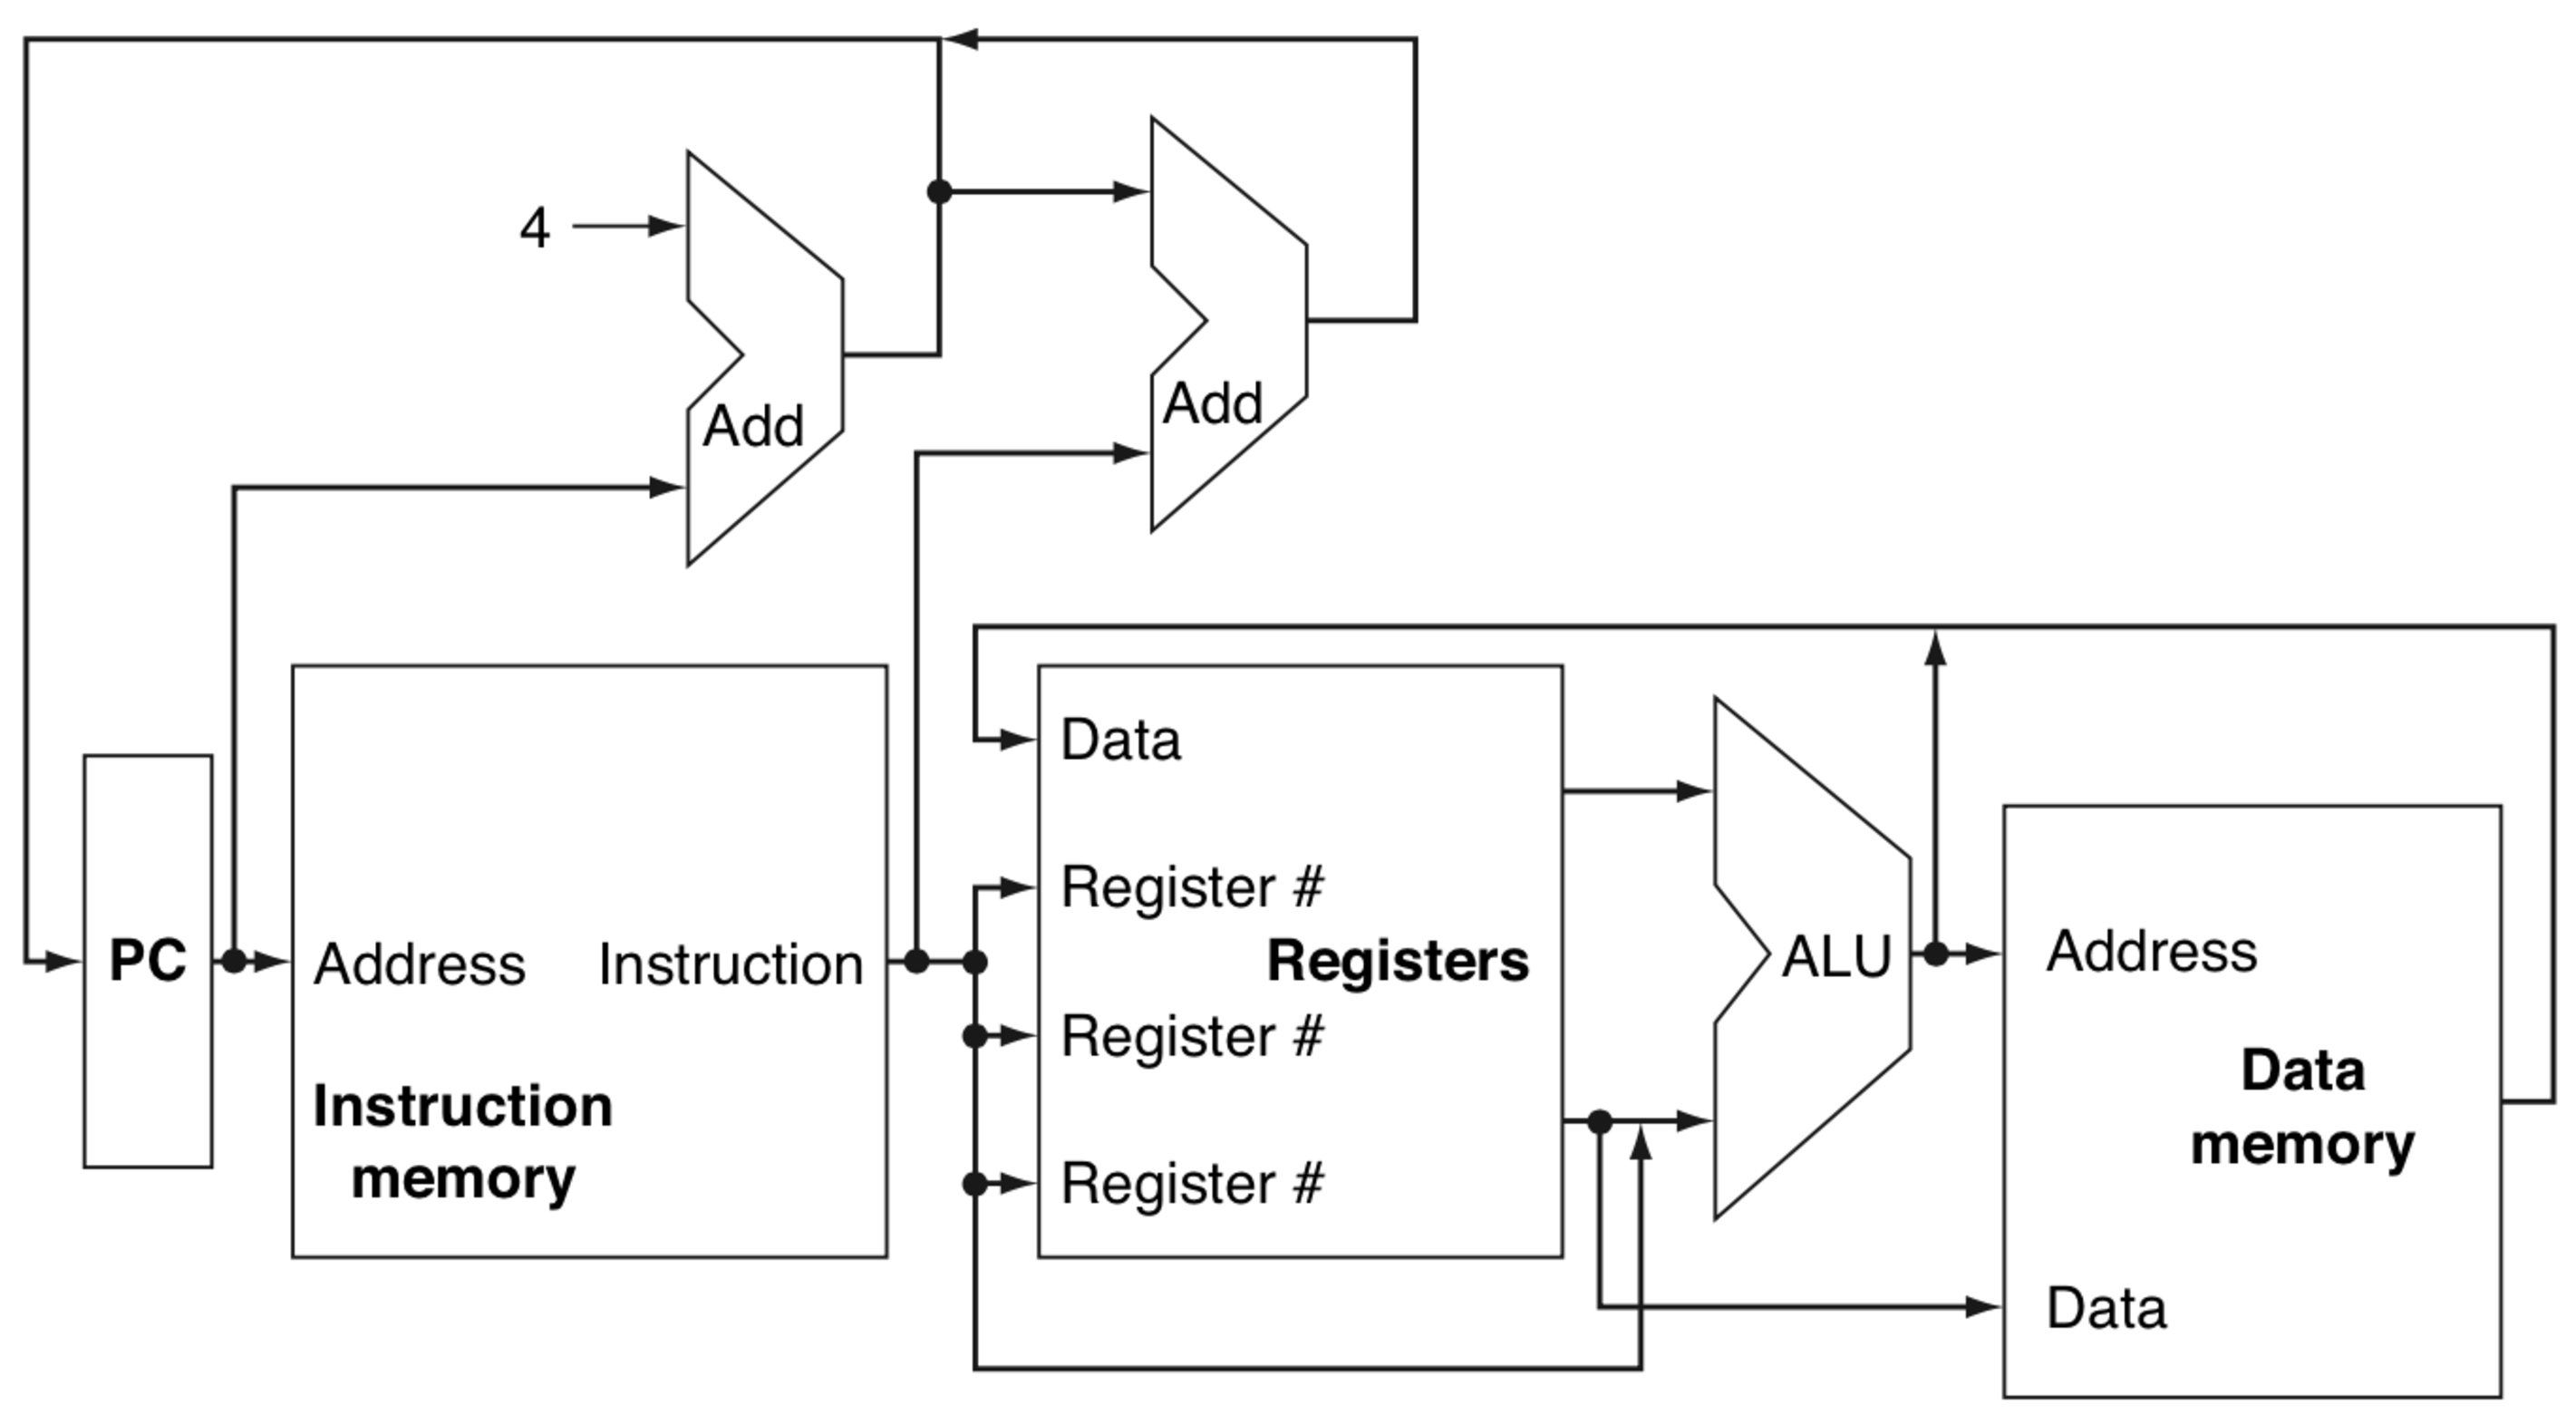
\includegraphics[width=6in]{./pics/mips-datapath}
\caption{An abstract (or high-level) view of a {\it MIPS} processor's datapath \cite{Patterson2005,Patterson2009}.}
\label{fig:mipsdatapath}
\end{figure}
%	Figure 4.1, Patterson2009, 4E, page 302
%	Figure 5.1, Patterson2005, 3E, page 287


Figure \ref{fig:mipsdatapath} shows the datapath of a simple, single-cycle microarchitectural implementation of the {\it MIPS} ISA. The datapath of a microarchitecture shows the hardware components, or logic circuits, needed to perform computation of arithmetic and logical operations as well as read/write data into memory. Its main components are logic circuits that: \vspace{-0.3cm}
\begin{enumerate} \itemsep -4pt
\item Fetch an instruction from memory, and update the program counter (PC).
\item Decode the instruction, and read register(s) (from the register file, {\tt regfile}) used by that instruction. The {\tt regfile} is shown as {\tt Registers} in Figure \ref{fig:mipsdatapath}.
\item Perform computation on an arithmetic/logical operation; i.e., the arithmetic-logical unit (ALU).
\item Read data from or write data to a memory device, or memory system (including caches). Separate memory devices can be used to store data and instructions separately. In Figure \ref{fig:mipsdatapath}, instruction memory is a memory device that stores instructions and data memory is another memory device that stores data. 
\end{enumerate}

These main components for the single-cycle microarchitectural implementation of the {\it MIPS} ISA are also used in other microarchitectural implementation of the {\it MIPS} ISA, such as the multi-cycle {\it MIPS} processor, pipelined {\it MIPS} processor, and the superscalar {\it MIPS} processor. The VLSI implementation of the main datapath components are briefly described as follows. The PC can be implemented as a binary counter or linear-feedback shift register that increments a binary number (either a 32- or 64- bit number) by four each clock cycle. A simple memory device for physical memory can be implemented using a dynamic random-access memory (DRAM). Alternatively, a simple memory system can be implemented with a three-level cache system and a DRAM, where a cache in either of the three levels can be implemented as a static random-access memory (SRAM). The ALU can be implemented with arithmetic circuits, such as adders, multipliers, and dividers. The ALU also includes comparators, shifters, one/zero detectors, encoders, and decoders \cite{Weste2011}. \\

Regarding the aforementioned design principles, I will discuss how this basic datapath satisfies the design principles mentioned earlier in Section \ref{sec:SingleCycleProcessorDesign}. Firstly, regularity in the {\it MIPS} ISA is found in majority of instructions that require the ALU to perform arithmetic or logic operations. This implies that a set of datapath components and a subset of the control logic can implement most instructions in the {\it MIPS} ISA. In addition, the regularity in the design of datapath components, such as adders in the ALU and DRAM devices, results in their simplicity. This allows architects to design simpler and faster datapaths that do not need to interface with complex control logic.  Secondly, as for smaller hardware components, components of the ALU (such as adders and shifters) are optimized for performance within area constraints. Also, for memory systems that include a multi-level cache system, the first level cache is designed to be smaller that the lower-level caches and the memory device. This allows the cache to be significantly faster than lower-level caches and the memory device. Thirdly, since most of the instructions use the ALU, a significant amount of work has been done to optimize ALU designs so that computer performance can be improved \cite{Ercegovac2004,Parhami2010,Stine2004,Farhat2004}. Lastly, the design trade-offs made for this simple datapath of a single-cycle {\it MIPS} processor demonstrates a trade-off between performance and hardware cost.




%%%%%%%%%%%%%%%%%%%%%%%%%%%%%%%%%%%%%%%%%%%
\subsection{Control Path Design for Single-Cycle Processors}
\label{ssec:ControlPathDesignforSingleCycleProcessors}

\begin{figure}[h]
\centering 
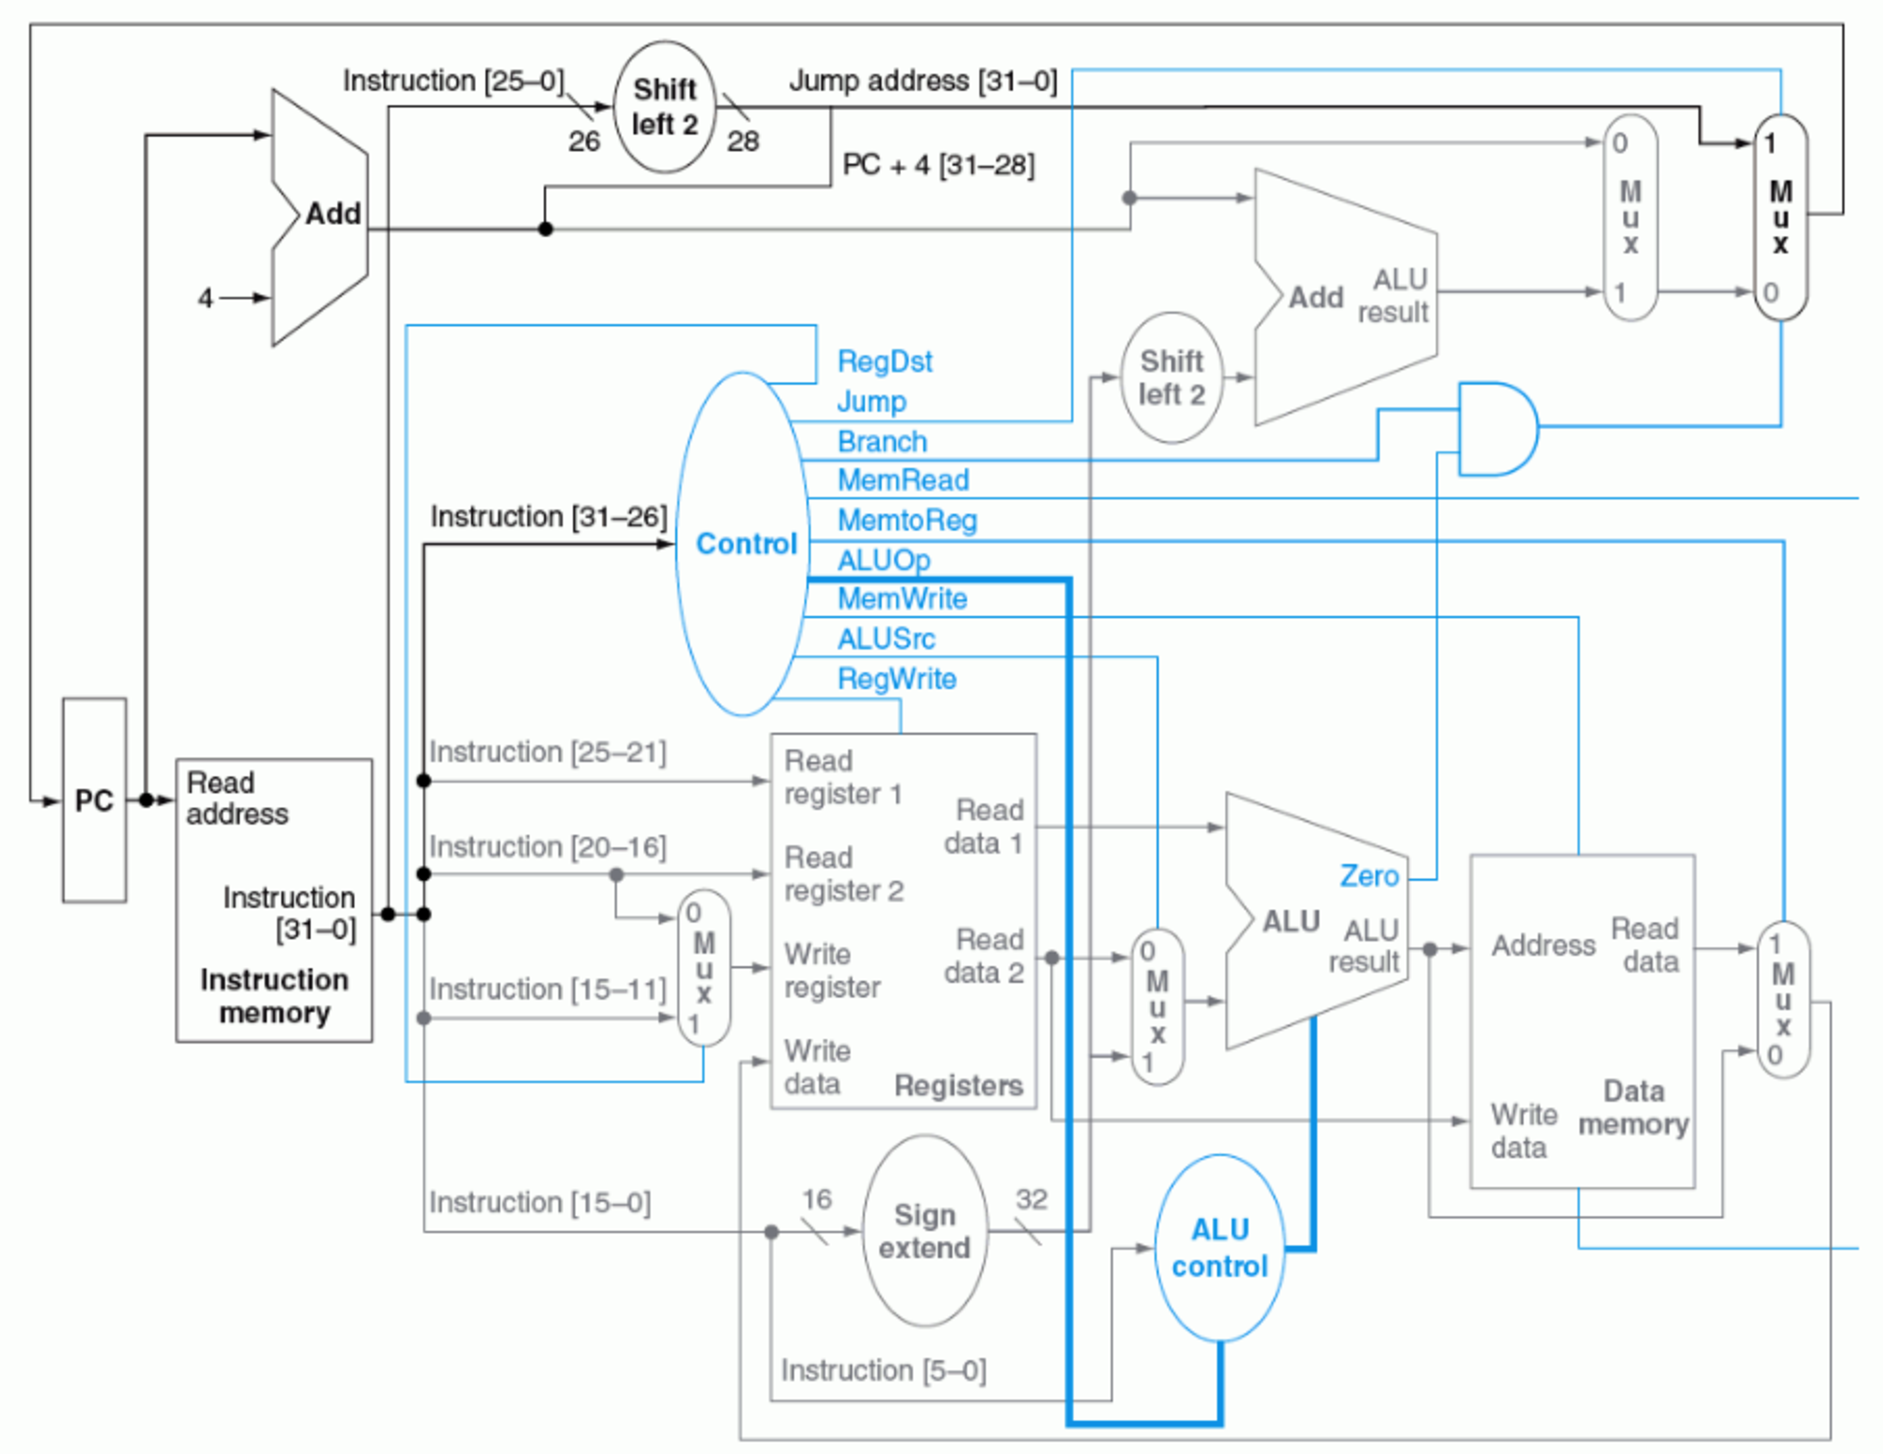
\includegraphics[width=5in]{./pics/single-cycle-processor}
\caption{Control path of a single-cycle {\it MIPS} processor, which is superimposed on the datapath of the {\it MIPS} processor \cite{Patterson2005,Patterson2009}.}
\label{fig:singlecycleprocessor}
\end{figure}
%	Figure 4.24, Patterson2009, 4E, page 329
%	Figure 5.24, Patterson2005, 3E, page 314

The control path of a processor includes a control unit to generate control signals for the processor, and wires to transmit those control signals from the control unit to various datapath components of the processor. This control unit for a single-cycle {\it MIPS} processor does not have multiple sequential states. Hence, the control unit can be implemented as a combinational logic circuit \cite{Patterson2005a}. \\

To implement the control unit as a combinational circuit, map the inputs of the control unit to its outputs. The mapping for a set of input signals to an output signal is a boolean function. This mapping can be represented as a truth table \cite{Patterson2005a} or a data structure that is typically used to represent a boolean function. Examples of such data structures include binary decision diagrams (BDDs)\cite{Hachtel1996,Hassoun2002} and AND-Inverter graphs (AIGs) \cite{Wang2009,BLSVG2011}. Electronic design automation (EDA) software can be used to optimize the size of truth tables, BDDs, or AIGs \cite{Wang2009}. By using EDA software to design and optimize the combinational circuit for the control unit, the process of designing the control path can be sped up by automation created by EDA software; also, EDA software can be used to automatically verify the correctness of the resultant circuits \cite{Scheffer2006,Scheffer2006a}. EDA software maps truth tables, BDDs, or AIGs to combinational circuits for the control unit. The combinational circuit for the control unit can be implemented as VLSI circuits using standard cells \cite{Kang2003a,Rabaey2003,Weste2011} or a programmable logic array (PLA) \cite{Patterson2005a}. \\

%The resultant hardware for the control unit is mapped by EDA software from the truth table, BDD, or AIG to a combinational circuit, using standard cells \cite{Kang2003a,Rabaey2003,Weste2011} or a programmable logic array (PLA) \cite{Patterson2005a}.





Figure \ref{fig:singlecycleprocessor} shows the datapath and the control path (in blue). The control path includes the control unit (shown as {\tt Control}) and ALU control unit {\tt ALU control}. The wiring of the buses and wires for the control path are colored in blue. The {\it PC} provides PC update, and the {\tt Instruction memory} fetches instructions from the memory device for instructions. The {\tt Registers regfile} allows data in registers to be read from the {\tt regfile}, and the lower {\tt ALU} provides computation of arithmetic and logical operations. The data memory allows data to be read from or written to memory \cite{Patterson2005,Patterson2009}. To summarize, sequentially ordered instructions from a software application would be loaded from memory into the processor for execution. After these instructions are executed, the resultant output data from executing those instructions would update the state of the processor. Next, data updated by the processor would be written to memory locations, or data would be read from memory. Finally, registers in the {\tt regfile} may have their data updated.



%%%%%%%%%%%%%%%%%%%%%%%%%%%%%%%%%%%%%%%%%%%
\subsection{Advantages and Disadvantages of Single-Cycle Processor Design}
\label{ssec:AdvantagesandDisadvantagesofSingleCycleProcessorDesign}

The single-cycle {\it MIPS} processor has the advantage of a simple datapath, which can be easily designed and verified. However, its major disadvantage is that it is computationally inefficient, since it requires all instructions to be executed in one clock cycle. Therefore, the CPI for the single-cycle {\it MIPS} processor is one. Since the latency of memory access instructions tends to be much slower than the latency of other instructions, the speed of the single-cycle {\it MIPS} processor is limited to the memory access speed \cite{Patterson2005,Patterson2009}.













































